\chapter{Introducción}

\section{Contexto y motivación}

Las simulaciones Monte Carlo son la herramienta estándar cuando la complejidad geométrica o la marcada anisotropía angular del flujo neutrónico dificultan la aplicación de métodos determinísticos. Sin embargo, cuando las partículas atraviesan blindajes o regiones altamente absorbentes, la estadística disponible en la zona de interés se reduce considerablemente, lo que incrementa la incertidumbre en magnitudes físicas clave como el flujo escalar o la dosis equivalente ambiental, e incluso puede imposibilitar su cálculo si no llega ninguna partícula. 

\emph{La incertidumbre estadística de estos resultados, por lo general, decrece lentamente con el número de historias simuladas, incrementando el costo computacional de forma prohibitiva.}

En este trabajo abordaremos la temática de la obtención de resultados a la salida de canales de extracción de neutrones en reactores de investigación tipo pileta. En estos sistemas, los neutrones generados en el núcleo deben atravesar el agua de la pileta antes de alcanzar la entrada del canal de extracción. Durante una simulación desde el núcleo, la mayoría de los neutrones permanecen dentro del mismo y aquellos que logran salir al agua son en gran medida absorbidos a medida que penetran en esta. En consecuencia, son escasos los neutrones que finalmente alcanzan la entrada del canal, haciendo que resulte computacionalmente costoso obtener estadística suficiente a la salida del canal, en el ambiente circundante o en dispositivos experimentales.

En la Figura \ref{fig:nucleo2} se presenta un esquema ilustrativo del núcleo de un reactor de investigación tipo pileta con un canal de extracción de neutrones. Este esquema consta de un núcleo central rodeado por agua y rodeado externamente por un blindaje biológico. El canal de extracción permite obtener un haz de neutrones destinado a usos posteriores en investigaciones experimentales. Además, se muestra esquemáticamente mediante un gradiente de color las regiones con mayor estadística neutrónica y cómo esta disminuye drásticamente al avanzar por el agua y el blindaje. Este esquema ejemplifica una simulación típica de núcleo, ilustrando claramente las dificultades que se tienen para obtener estadística lejos del núcleo.

\begin{figure}[H]
    \centering
    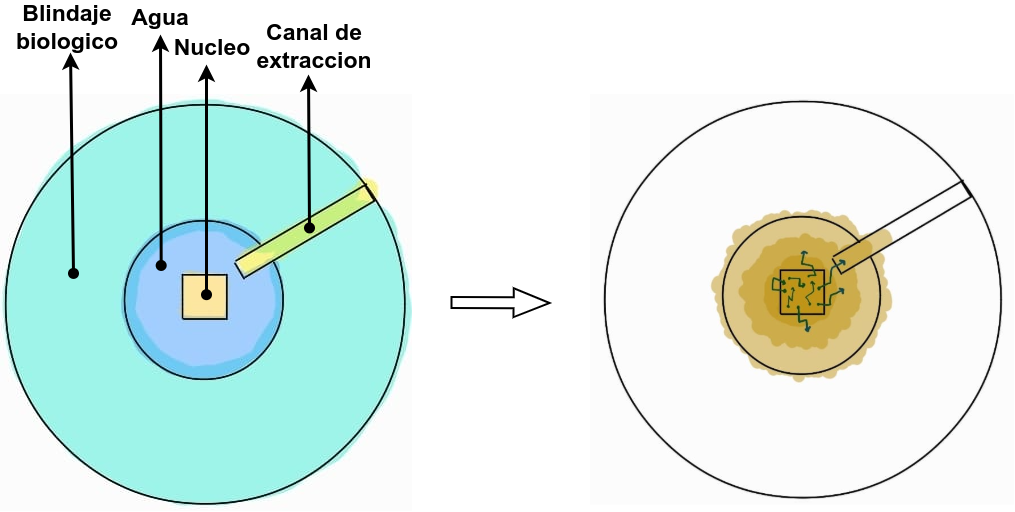
\includegraphics[width=0.8\textwidth]{nucleo2.png}
    \caption{Representación esquemática del núcleo de un reactor tipo pileta con canal de extracción. Se observa el núcleo central, rodeado por agua y blindaje biológico, así como un canal de extracción de neutrones. El gradiente de color indica cualitativamente la distribución de la población neutrónica típica en simulaciones Monte Carlo desde el núcleo.}
    \label{fig:nucleo2}
\end{figure}


% Para mitigar esta problemática, se emplean técnicas de reducción de varianza. Entre ellas, destaca el método general del \emph{source biasing}, basado en re-muestrear las fuentes originales. Esta técnica consiste en reemplazar la distribución original de partículas por una estadísticamente equivalente, construida sobre una superficie intermedia estratégicamente seleccionada. De esta manera, las partículas transportadas tienen mayor probabilidad de contribuir eficientemente a los tallies seleccionados, mejorando la estadística en la región objetivo sin aumentar desproporcionadamente el tiempo de CPU.

Para mitigar esta problemática, se suelen emplear técnicas de reducción de varianza tales como:
\begin{itemize}

    \item \textbf{Separación geométrica del problema}: consiste en dividir la simulación en regiones contiguas, separando la fuente original de la región de interés mediante una superficie de interfaz. En esta superficie se registra la distribución de partículas en el espacio de fases y su peso estadístico. Esta información se emplea para construir una nueva fuente que se utiliza en una simulación posterior, permitiendo focalizar los recursos computacionales exclusivamente en la región de interés.
    
    \item \textbf{Ventanas de peso}: esta técnica define un rango aceptable de pesos estadísticos para las partículas en cada región del dominio. Aquellas con peso muy alto son divididas (\emph{splitting}) y las de peso muy bajo pueden ser descartadas con cierta probabilidad, controlando así la varianza espacialmente.
    
    \item \textbf{Ruleta rusa}: se utiliza para descartar partículas con bajo peso estadístico, preservando el valor esperado del cálculo. Cada partícula tiene una probabilidad de ser eliminada o de continuar con su peso ajustado en consecuencia.
    
    \item \textbf{Sesgo por supervivencia}: en lugar de eliminar partículas cuando son absorbidas, se les reduce su peso estadístico de acuerdo a la probabilidad de absorción, permitiendo que las partículas sobrevivan y continúen su historia.
\end{itemize}

% En este trabajo se desarrolló una técnica basada en la separación geométrica del problema, con el objetivo de restringir la simulación a la región de interés. Para ello, se establece una superficie de acople ubicada estratégicamente dentro del modelo, sobre la cual se registran un archivo de partícula generado durante una simulación inicial que abarca el núcleo del reactor. Este archivo permite construir una fuente distribucional que reproduce de forma estadísticamente equivalente las distribuciones originales en el espacio de fases ($\mathbf{E}$–$\mathbf{r}$–$\boldsymbol{\Omega}$), incluyendo también el peso estadístico de cada partícula.

% A continuación, se genera una nueva simulación que consiste en la región de interés, utilizando la fuente distribucional como fuente ubicada en la superficie de acople. Al concentrar el computo en la zona de interes se incrementa la eficiencia, ya que las partículas simuladas poseen una mayor probabilidad de contribuir efectivamente a las magnitudes físicas relevantes de estudio, sin necesidad de transportar todo el sistema desde la fuente original de núcleo.

% En particular, en este trabajo se desarrolla una técnica basada en la separación geométrica del problema, cuyo objetivo es desacoplar geometricamente el modelo, restringiendo la simulación a la región de interés. Para ello, se establece una superficie de acople en una ubicación intermedia dentro del modelo, sobre la cual se registra un archivo de partículas generado durante una simulación inicial. A partir de este archivo, se construyen una fuente distribucional que reproduce de forma estadísticamente equivalente las distribuciones originales en el espacio de fases. De esta manera, en la etapa subsiguiente se generan partículas directamente en la región de interés, aumentando la eficiencia del cálculo, sin necesidad de transportar todo el sistema desde el núcleo.

%  En particular, en este trabajo se utiliza una implementación que consiste en desplazar virtualmente la fuente original hacia posiciones intermedias más cercanas al área de interés. Esto se logra mediante la grabación de archivos de partículas (\textit{trackfiles}) en superficies estratégicamente ubicadas durante la simulación inicial, los cuales permiten luego construir fuentes sintéticas denominadas fuentes de distribucionales que poseen distribuciones estadísticamente equivalentes a las originales. De esta manera, las partículas generadas en etapas subsiguientes poseen una mayor probabilidad de contribuir a los tallies definidos, mejorando la estadística en la región de estudio sin aumentar desproporcionadamente el tiempo de \textit{CPU}.

% \section{Fuentes distribucionales – base conceptual}

% El método se implementa dividiendo el problema original en una sucesión de etapas consecutivas delimitadas por \emph{superficies de acople} $\{\mathcal{S}_{i}\}_{i=1}^{\,n-1}$. Durante cada etapa $i$, se simulan partículas desde la fuente original hasta la superficie $\mathcal{S}_{i}$, almacenándose las propiedades de cada partícula (\emph{tracks}) en el espacio de fases ($\mathbf{E}$–$\mathbf{r}$–$\boldsymbol{\Omega}$) y su peso estadístico. Estas superficies se definen en posiciones donde sea posible registrar suficientes partículas para construir una fuente secundaria representativa en un tiempo razonable.

% El método se implementa dividiendo el problema original en una sucesión de etapas consecutivas delimitadas por \emph{superficies de acople} ${\mathcal{S}{i}}{i=1}^{,n-1}$. En la primera etapa, las partículas se simulan directamente desde la fuente original hasta la superficie $\mathcal{S}{1}$, registrando sus propiedades (o \emph{tracks}) en el espacio de fases ($\mathbf{E}$–$\mathbf{r}$–$\boldsymbol{\Omega}$) junto con su peso estadístico. A partir de estos datos, se construye una fuente secundaria representativa en dicha superficie, la cual se emplea como condición inicial en la etapa siguiente. Así, en cada etapa $i > 1$, las partículas no se simulan desde la fuente original, sino desde una fuente sintetizada en la superficie $\mathcal{S}{i-1}$, desplazando progresivamente la fuente hacia la región de interés. Las superficies de acople se ubican en posiciones estratégicas donde sea posible registrar una estadística suficiente en un tiempo computacional razonable.

% A partir de las listas generadas, se estima la distribución multidimensional de las partículas en la superficie $\mathcal{S}_{i}$, preservando las correlaciones entre las variables mencionadas. Esta distribución estimada se utiliza luego como fuente inicial en la siguiente etapa ($i+1$). De este modo, la fuente se traslada progresivamente hacia la región objetivo, logrando la precisión requerida con un número considerablemente menor de historias que el método tradicional sin reducción de varianza.

El método desarrollado en este trabajo se basa en la separación geométrica del problema en dos regiones: una que contiene el núcleo del reactor, y otra que abarca exclusivamente la región de interés. Esta técnica se implementa mediante la división del modelo simulado en dos regiones, delimitadas por superficies de acople ubicadas estratégicamente dentro de la geometría. En una primera etapa, se realiza una simulación completa del núcleo hasta una superficie intermedia, donde se registran en una lista las propiedades de las partículas que la atraviesan, incluyendo su energía, posición, dirección ($\mathbf{E}$–$\mathbf{r}$–$\boldsymbol{\Omega}$), y su peso estadístico.

A partir de esta lista de partículas, se estima la distribución multidimensional en el espacio de fases utilizando histogramas multidimensionales. Esta estructura permite segmentar el conjunto original de datos mediante histogramas de baja resolución, llamados histogramas macro, que separan el espacio de fases en regiones donde las correlaciones entre variables se mantienen aproximadamente constantes. Sobre cada una de estas regiones, se construyen histogramas de mayor resolución —los histogramas micro— que aproximan la distribución de cada variable con mayor detalle. De este modo, se preservan tanto la forma general de la distribución como las correlaciones relevantes entre las variables registradas. A partir de esta estimación, es posible generar nuevas partículas que pertenezcan estadísticamente al mismo espacio de fases que la muestra original, obteniendo así una fuente sintética denominada fuente distribucional. Esta metodología se desarrolla en profundidad en el Capítulo \ref{cap:metodo_histogramas}, donde se describe el procedimiento implementado para su construcción.

% A partir de esta lista de partículas, se estima la distribución multidimensional en el espacio de fases utilizando histogramas multidimensionales jerárquicamente acoplados. Esta estructura permite preservar las correlaciones entre variables a través de un orden preestablecido de procesamiento, generando así una fuente sintética denominada fuente distribucional.

En la segunda etapa, esta fuente distribucional se utiliza como fuente de entrada para una nueva simulación, que consiste únicamente en la región de interés, excluyendo el núcleo y sus alrededores. Al concentrar el esfuerzo computacional en esta zona, se incrementa la eficiencia, ya que las partículas simuladas poseen una mayor probabilidad de contribuir a las magnitudes físicas relevantes de estudio.

\emph{A su vez, además del método mencionado, en este trabajo también se hace uso del método de \textbf{ventanas de peso} como técnica complementaria de reducción de varianza.}

% El método consiste en dividir el problema en una sucesión de etapas consecutivas, delimitadas por superficies de acople, ubicadas estratégicamente a lo largo de la geometría simulada. En la primera etapa, las partículas se simulan desde la fuente original hasta la primer superficie, donde se registran sus propiedades en el espacio de fases ($\mathbf{E}$–$\mathbf{r}$–$\boldsymbol{\Omega}$) en un archivo denominado \textit{trackfile}. A partir de esta lista de partículas, se aproxima la distribución multidimensional preservando las correlaciones entre las variables, y se utiliza para generar una fuente secundaria en dicha superficie. Esta fuente es entonces utilizada en la siguiente etapa. El proceso se repite, trasladando progresivamente la fuente hacia la región de interés. 

En la Figura \ref{fig:nucleo4} se ejemplifica el proceso desarrollado para una simulación del núcleo de un reactor de investigación tipo pileta. Inicialmente, se realiza una simulación completa desde el núcleo, obteniendo una estadística adecuada en los alrededores del mismo, la cual se reduce considerablemente a medida que los neutrones penetran en el agua circundante. Este fenómeno se visualiza mediante un gradiente de colores. En esta simulación inicial, se define una superficie de registro en la entrada de un canal de extracción. Las partículas que atraviesan dicha superficie se registran en un archivo de partículas, el cual, mediante la metodología que se va a desarrollar en este trabajo, se procesa para definir una fuente distribucional. Posteriormente, esta fuente permite simular únicamente el canal de extracción, concentrando la estadística en dicha región sin necesidad de repetir la simulación completa desde el núcleo.

\begin{figure}[H]
    \centering
    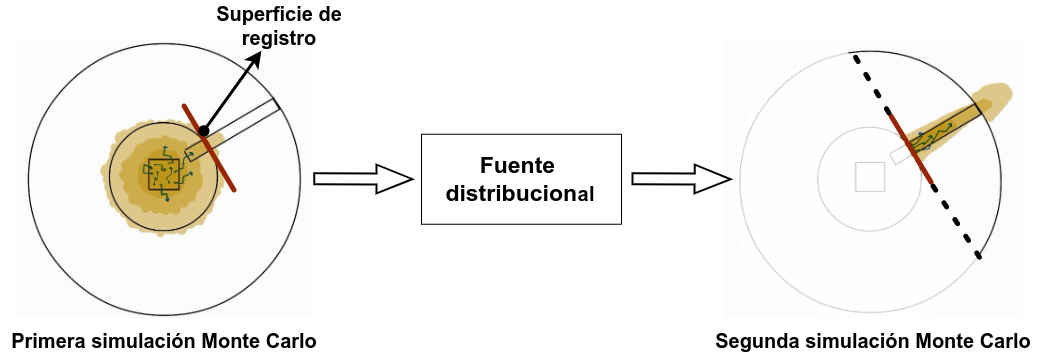
\includegraphics[width=\textwidth]{nucleo4.png}
    \caption{Esquema ilustrativo del proceso de desacople geométrico en simulaciones Monte Carlo para un reactor de investigación tipo pileta. En la primera etapa se registra un archivo de partículas en la entrada del canal de extracción, el cual es posteriormente utilizado para generar una fuente distribucional que permite simular eficientemente el canal de forma independiente. El gradiente de colores representa la disminución de la población neutrónica.}
    \label{fig:nucleo4}
\end{figure}

\emph{Este enfoque permite alcanzar una buena precisión en zonas alejadas o poco accesibles, con un número considerablemente menor de historias simuladas en comparación con una simulación completa desde la fuente original.}

En resumen, el procedimiento consta de tres etapas fundamentales:

\begin{itemize}
    \item \textbf{Detección}: Registro de las variables del espacio de fases y del peso estadístico de cada partícula que atraviesa una superficie intermedia de desacople. El resultado de este proceso es un archivo de partículas que contiene la información necesaria para caracterizar la distribución de la fuente sobre dicha superficie.

    \item \textbf{Estimación}: Procesamiento del archivo de partículas mediante la metodología propuesta en este trabajo, basada en histogramas multidimensionales. Este procedimiento permite aproximar la distribución en el espacio de fases, preservando las correlaciones entre variables, y genera como resultado una fuente distribucional.

    \item \textbf{Producción}: Utilización de la fuente distribucional estimada para generar nuevas partículas que pertenezcan al espacio de fases del archivo de partículas original. Estas partículas son empleadas en simulaciones posteriores, permitiendo modelar la región de interés de forma desacoplada de la fuente original.
\end{itemize}

El archivo original de partículas contiene inevitablemente regiones del espacio de fases con baja estadística o sin eventos registrados, producto de su carácter finito. Si se reutiliza directamente como fuente en una simulación posterior —por ejemplo, simulando varias veces las mismas partículas registradas— se corre el riesgo de reproducir el mismo ruido estadístico, afectando la calidad de los resultados.

Para mitigar este problema, se emplea un procedimiento de estimación basado en histogramas multidimensionales que permite densificar el espacio de fases. En este enfoque, se utilizan histogramas para aproximar la distribución de variables, bajo el supuesto de que la probabilidad es constante dentro de cada bin. Esto habilita la generación de nuevas partículas en regiones que no estaban presentes explícitamente en el archivo original, completando así los vacíos estadísticos y asegurando una cobertura más uniforme del espacio de fases.

\section{Trabajos relacionados}

Los trabajos previos realizados en el Departamento de Física de Reactores y Radiaciones (DeFRRa) del Centro Atómico Bariloche (CAB) abordaron el modelado de fuentes distribucionales mediante el uso de histogramas multidimensionales \cite{Fairhurst2017Hist, Ayala2019Hist, Abbate2020Hist}. Esta estrategia permitió capturar correlaciones entre energía, posición y dirección en geometrías planas rectangulares, siendo aplicada satisfactoriamente en estudios vinculados al reactor RA‑10.

En continuidad con dichos desarrollos, la herramienta \texttt{KDSource} —también desarrollada en el DeFRRa— introdujo técnicas más avanzadas basadas en \textit{Kernel Density Estimation} (\textit{KDE}), en forma multivariante y adaptativa \cite{Abbate2021KDSource, Schmidt2022KDSourcePaper, Fox2022KDE, Gimenez2024KDSourceOpenMC}. \texttt{KDSource} permite ajustar automáticamente distribuciones continuas a partir de archivos de partículas previamente obtenidos y, a partir de ellas generar fuentes distribucionales, preservando las correlaciones del espacio de fases.

No obstante, el enfoque basado en \textit{KDE} presenta una limitación: su carácter inherentemente suavizante puede dificultar la representación precisa de discontinuidades abruptas en el espacio de fases. Estas discontinuidades pueden originarse, por ejemplo, en zonas de cambio de material o en la coexistencia de poblaciones de partículas con comportamientos físicos muy distintos, como neutrones térmicos isotrópicos mezclados con neutrones rápidos colimados. En estos casos, la suavización puede degradar la calidad de la fuente generada, especialmente cuando se busca preservar estructuras finas o anisotropías marcadas.

El presente trabajo extiende estas líneas incorporando los enfoques basados en histogramas multidimensionales dentro del entorno ya establecido de \texttt{KDSource}, proponiendo además un método de discretización adaptativa que automatiza la definición de las grillas de los histogramas macro y micro. A diferencia de los trabajos anteriores, este nuevo enfoque permite segmentaciones variables para diferentes subconjuntos del espacio de fases. Por ejemplo, el método puede asignar una discretización espacial más refinada para neutrones rápidos, donde suelen prevalecer anisotropías asociadas a haces colimados, y una discretización más homogénea para neutrones térmicos, cuya distribución tiende a ser más isotrópica. De esta forma, se logra preservar las correlaciones relevantes sin imponer una malla uniforme en todo el dominio, mejorando la capacidad de representación del método.

% No obstante, \textit{KDE} presenta una desventaja: su carácter inherentemente suavizante puede reducir la capacidad de representar adecuadamente discontinuidades abruptas presentes en ciertos problemas físicos relevantes.

% El presente trabajo extiende estas líneas incorporando los enfoques basados en histogramas multidimensionales dentro del entorno ya establecido de \texttt{KDSource}, proponiendo además un método de discretización adaptativa que automatiza la definición de las grillas de los histogramas macro y micro. A diferencia de los trabajos anteriores, este nuevo enfoque permite segmentaciones variables para diferentes subconjuntos del espacio de fases original. Por ejemplo, neutrones térmicos y rápidos pueden ser tratados con distinta resolución espacial, asignando automáticamente histogramas macros diferenciados en función de su energía. De forma análoga, la adaptabilidad también se extiende a los histogramas micro, permitiendo una resolución de la aproximación de las distribuciones condicionada por otras variables.

% Los desarrollos previos en el Departamento de Física de Reactores y Radiaciones (DeFRRa) del Centro Atómico Bariloche (CAB) han empleado histogramas anidados con discretización gruesa y fina (macro/micro-bins) para capturar adecuadamente las correlaciones entre energía, posición y dirección en fuentes planas rectangulares. Si bien este enfoque permitió resolver satisfactoriamente casos específicos relacionados con el reactor RA‑10, presenta limitaciones. Entre ellas, destacan la necesidad de definir manualmente las grillas de discretización, la poca suavidad inherente a los histogramas y las dificultades para tratar correctamente discontinuidades abruptas, como aquellas generadas por cambios de material o geometría.

% Posteriormente, la herramienta \texttt{KDSource} —desarrollada también en el DeFRRa— introdujo el uso de técnicas más avanzadas basadas en \textit{Kernel Density Estimation} (\textit{KDE}) multivariante adaptativa. El flujo de trabajo de \texttt{KDSource} comprende dos etapas diferenciadas: (i) una fase inicial de optimización \emph{off-line}, en la cual se ajusta automáticamente el modelo \textit{KDE} a partir de \textit{trackfiles} preexistentes, y (ii) una fase de muestreo \emph{on-the-fly}, donde un módulo integrado en \texttt{C}/\texttt{C++} genera nuevas partículas durante la simulación Monte Carlo manteniendo las correlaciones globales y la normalización del peso original. Este enfoque elimina la necesidad de manejar \textit{trackfiles} voluminosos durante la simulación, optimizando sustancialmente el uso de memoria \textit{RAM}.

% \begin{figure}[H]
%     \centering
%     
\includegraphics[width=0.5\textwidth]{figs/kdsource_logo.png}
%     \caption{Logo de \texttt{KDSource}. Fuente: \url{https://kdsource.readthedocs.io/en/latest/}}
%     \label{fig:kdsource_logo}
% \end{figure}



\section{Aportes específicos de este trabajo}

Este trabajo busca profundizar el desarrollo de \texttt{KDSource} mediante la incorporación de histogramas multidimensionales como una alternativa -o complemento- a la metodología \textit{KDE} existente. Las contribuciones específicas son:

\begin{itemize}
    \item Implementación de histogramas multidimensionales en \texttt{KDSource}, capaces de:
    \begin{itemize}
        \item preservar las correlaciones entre variables ($\mathbf{E}$–$\mathbf{r}$–$\boldsymbol{\Omega}$) para fuentes planas rectangulares;
        \item representar adecuadamente discontinuidades o picos en todas las variables;
        \item implementar un método de selección automática y adaptativa de bordes para los histogramas, tanto a nivel macro como micro, optimizado según la estadística disponible en cada subgrupo del espacio de fases.
    \end{itemize}

    \item Integración optimizada del flujo de trabajo en \texttt{OpenMC} mediante:
    \begin{itemize}
        \item generación \emph{offline} de un archivo intermedio en formato \texttt{XML} conteniendo la fuente distribucional, que incluye la información de los histogramas multidimensionales;
        \item desarrollo de un módulo en \texttt{C} que utilice eficientemente esta información para producir partículas individualmente;
        \item implementación de un remuestreo \emph{on-the-fly} integrado directamente en \texttt{OpenMC}, minimizando la ocupación de memoria al evitar la carga y gestión de archivos extensos de partículas.
    \end{itemize}

    \item Validación  del método en casos de complejidad creciente:
    \begin{itemize}
        \item Un caso simplificado, consistente en un haz colimado ingresando en un paralelepípedo de agua atravesado por un canal de vacío, con fuentes definidas artificialmente para permitir una comparación con una simulación directa más extensa sin la aplicación del método desarrollado. 
        \item Un caso real, consistente en la propagación a través del conducto Nº5 del reactor RA‑6, utilizando un archivo de partículas proporcionada por el departamento de Física de Neutrones del CAB generada a través de una simulación del núcleo en \texttt{OpenMC}.
    \end{itemize}
\end{itemize}




% \chapter{Introducción}

% \section{Contexto y motivación}

% Las simulaciones de transporte por metodo Monte Carlo son la herramienta de referencia cuando 
% la geometría y/o la anisotropía angular hacen inviables los métodos determinísticos. 
% Sin embargo, a medida que las partículas atraviesan blindajes o regiones muy absorbentes,
%  la estadística en la zona de interés se vuelve escasa y la incertidumbre de tallies, como
%   el flujo escalar por ejemplo, escala de forma prohibitiva con el tiempo de simulacion.
%   Para reducir el error estadistico sin multiplicar el tiempo de CPU se recurre a técnicas de 
%   reducción de varianza. Una de las más 
%    utilizadas es el re-muestreo de fuentes (source biasing en sentido amplio), 
%    donde se reemplaza la fuente original por una distribución estadísticamente 
%    equivalente construida en una superficie intermedia. De este modo se transportan 
%    preferentemente las partículas con mayor probabilidad de contribuir a los tallies 
%    seleccionados.

% \section{Fuentes distribucionales – base conceptual}


% La metodología se lleva a la práctica dividiendo el problema original 
% en $n$ etapas de transporte contiguas, delimitadas por \emph{superficies 
% de acople} $\{\mathcal{S}_{i}\}_{i=1}^{\,n-1}$. Durante la etapa $i$ se 
% simulan todas las partículas desde la fuente hasta la superficie 
% $\mathcal{S}_{i}$ y se guarda la \emph{lista de tracks} asociada, es decir, 
% el vector de fase de cada partícula que atraviesa la superficie. 
% Estas superficies se eligen de modo que el número de tracks registrado 
% resulte estadísticamente representativo para construir una fuente secundaria 
% confiable.


% A partir de cada lista se obtiene una estimación de la distribución multidimensional de 
% las partículas sobre $\mathcal{S}_{i}$ —conservando las correlaciones entre energía, posición 
% y dirección— y esa distribución se utiliza como fuente al comenzar la etapa $i\!+\!1$. Así, 
% la fuente efectiva se relocaliza paso a paso hacia la región de detección y se alcanza la 
% precisión deseada con un número de historias considerablemente menor que el requerido en un 
% cálculo sin \emph{source biasing}.



% El procedimiento completo consta de tres etapas:

% \begin{itemize}
%     \item \textbf{Detección} – Se registran las partículas (tracks) que cruzan una 
%     superficie intermedia de desacople, la cual actúa como desacople entre las distintas etapas de la simulación Monte Carlo, y se almacenan sus coordenadas en el espacio de fases 
%     ($E$, $x$, $y$, $\mu$, $\phi$, peso).
%     \item \textbf{Estimación} – A partir de esa lista se aproxima la distribución 
%     conjunta y sus correlaciones.
%     \item \textbf{Producción} – Se muestrea esa distribución para generar tantas 
%     partículas como sea necesario en la simulación secundaria.
% \end{itemize}

% Los primeros desarrollos en el Departamento de Física de Reactores y Radiaciones emplearon
% histogramas anidados (macro/micro–bins) para capturar las correlaciones
% $E$–$x$–$y$–$\mu$–$\phi$ en fuentes planas rectangulares.  
% Si bien el método permitió resolver algunos casos de aplicación
% presentados en tesis previas vinculadas al RA‑10, la definición manual
% de grillas y la limitada suavidad de las curvas generadas plantean
% desafíos cuando aparecen discontinuidades fuertes —por ejemplo, en cambios
% bruscos de material a través de una interfase— y al trasladarlo a otras
% geometrías.

% KDSource —una herramienta creada en el DFRyR para el post‑procesamiento
% y re‑muestreo de listas de partículas— emplea desde su concepción la
% \textit{Kernel Density Estimation} (KDE) multivariante adaptativa.
% El flujo de trabajo estándar consta de dos etapas: (i) optimización
% \emph{off‑line}, donde a partir de la lista de tracks se ajusta un
% modelo KDE con selección automática de ancho de banda, y (ii) muestreo
% \emph{on‑the‑fly}, en el cual un módulo en \texttt{C}/\texttt{C++}
% integra ese modelo dentro del código Monte Carlo y genera
% partículas una a una, conservando las correlaciones globales
% $E$–$\mathbf{r}$–$\boldsymbol{\Omega}$ y la normalización original del peso.
% Gracias a esta separación, KDSource elimina la necesidad de manipular
% archivos voluminosos de tracks durante la simulación. No obstante, el carácter suavizante de
% KDE puede atenuar discontinuidades muy marcadas; por ello este trabajo
% propone un esquema de histogramas multidimensionales adaptativos que
% mantenga las ventajas del muestreo continuo pero ofrezca un control
% más explícito sobre la resolución local.

% \section{Aportes específicos de este trabajo}

% El proyecto profundiza el desarrollo de KDSource mediante la
% incorporación de histogramas multidimensionales adaptativos como
% alternativa —o complemento— a KDE, con el objetivo de reproducir con
% mayor fidelidad estructuras espectrales o espaciales abruptas sin perder
% la correlación global entre variables.

% \begin{itemize}
%     \item Implementar un método alternativo de histogramas multidimensionales adaptativos dentro de KDSource que:
%     \begin{itemize}
%         \item reproduzca adecuadamente las correlaciones $E$-$x$-$y$-$\mu$-$\phi$ en una fuente plana rectangular perpendicular al eje $z$;
%         \item conserve las discontinuidades espectrales y espaciales propias de interfaces o colimadores;
%         \item ofrezca un control explícito del compromiso resolución/estadística.
%     \end{itemize}
    
%     \item Integrar y optimizar el flujo de trabajo en \texttt{OpenMC}:
%     \begin{itemize}
%         \item Generar, en modo off-line, un archivo intermedio (XML + HDF5) que contiene los histogramas y metadatos de la distribución.
%         \item Construir un módulo en C que, utilizando esa información, produzca una partícula a la vez.
%         \item Integrar el muestreo directamente en el código fuente de OpenMC (modo on-the-fly), de forma que sólo se mantenga en RAM la información de los histogramas y se evite la creación y carga de listas voluminosas.
%     \end{itemize}
    
%     \item Validar la herramienta en dos etapas de dificultad creciente:
%     \begin{itemize}
%         \item un caso simplificado: haz colimado que ingresa en un paralelepípedo
%         de agua atravesado por un canal de vacío; la fuente en la entrada
%         del conducto es definida y muestreada libremente, lo que permite
%         comparar los resultados con una simulación directa sin reducción
%         de varianza;
%         \item un caso condicionado por la fuente: propagación, a lo largo del
%         conducto N.º 5 del RA‑6, de la lista de partículas obtenida por el
%         Grupo de Física de Neutrones a partir de una simulación de núcleo;
%         aquí la estadística está limitada por la lista original y se
%         evalúa el desempeño del método bajo esa restricción.
%     \end{itemize}
% \end{itemize}
